\documentclass{article}
\usepackage{titling}
\usepackage{enumitem} 
\usepackage{tikz}
\usepackage{listings}
\usepackage{nameref}
\usepackage{hyperref}
\usepackage{float}
\restylefloat{table}

\usetikzlibrary{arrows,positioning,calc}


\usepackage[utf8]{inputenc}

%\setlength{\droptitle}{-10em} 

\title{PAK: Report 2}
\author{Nikolai Tschacher  \\
	Humboldt-Universität zu Berlin, Germany  \\
	tschachn@hu-berlin.de}

\date{\today}
% Hint: \title{what ever}, \author{who care} and \date{when ever} could stand 
% before or after the \begin{document} command 
% BUT the \maketitle command MUST come AFTER the \begin{document} command! 
\begin{document}

\maketitle


%\begin{abstract}
%Short introduction to subject of the paper \ldots 
%\end{abstract}

\section{Introduction} 
In this report we are going to research the fairness between different combinations of TCP-Variants (especially their congestion mechanism). We will build a simple network topology consisting of four distinct nodes. There will be one bottleneck link in the topology. Two given TCP-Variants will compete for this bottleneck link. The simple topology is illustrated in figure \ref{fig:simpleYtopology}. We chose to compare two TCP New Reno and two Cubic connections. We will simulate TCP traffic over the bottleneck link using the network simulator NS-3. We are going to use version 3.26 in this report.

\begin{figure}[H]
\centering
\let\clearpage\relax
\tikzset{
    >=stealth',
    n0de/.style={
           circle, 
           draw=black,
           minimum size=1cm,
           text centered},
}

\begin{tikzpicture}[every node/.style={},auto,>=latex']

\node[n0de](A){A};
\node[n0de, below=1cm of A](B){B};
\node[n0de](R)[right= 1cm of {$(A)!0.5!(B)$}]{R};
\node[n0de](C)[right= 1cm of R]{C};

\path[->] (A)  edge node {$L1$} (R);
\path[->] (B)  edge node {$L2$} (R);
\path[->] (R) edge node {$b$} (C);


\end{tikzpicture}

\caption{Two network nodes (A and B) sent traffic over the bottleneck \textit{b} to the sink C} \label{fig:simpleYtopology}
\end{figure}

\section{Analysis} \label{analysis}
\let\clearpage\relax
In the following section we will include the mathematical models underlying our simulation. Let $L1, L2, b$ be the data rates of the corresponding links in figure \ref{fig:simpleYtopology}. The latency on all links is variable. The MSS is equal for the two TCP-Connections. Package loss is introduced on both interfaces of link b. We make use of a error model where packets get lost according a uniform random distribution. The rate of one TCP connection is:

$$R = \sqrt{\frac{3}{2} \cdot \frac{1}{p}} \cdot \frac{MSS}{RTT}$$

When we put the rates of our TCP connections into relation we get:

$$\frac{R_A}{R_B} = \frac{\sqrt{\frac{3}{2} \cdot \frac{1}{p}} \cdot \frac{MSS}{RTT_A}}{\sqrt{\frac{3}{2} \cdot \frac{1}{p}} \cdot \frac{MSS}{RTT_B}} = \frac{RTT_B}{RTT_A} $$

The equation above puts the fraction of the achieved throuput in relation to their RTT. We see that the fraction of throuput is reversly proportional to their RTTs.

\section{Simulation} \label{simulation}
Our simulation script is written in \emph{C++} and implemented within the discrete network simulator \emph{ns-3}. Our implementation source code are attached in the appendix.

\paragraph{General assumptions:} The links $L1, L2$ send packets with a constant rate of 5Mbps. The RTT on $L1, L2$ may vary, we will simulate all latency combinations with latencys $(5ms, 10ms, 20ms, 50ms)$. Sender nodes (A and B) are sending packet frames  with a length of 1502 bytes (zero-byte arrays as TCP payload).\\\\
The bottleneck link $b$ has a bandwith of 2Mbps, which is roughly half the bandwith of the links $L1, L2$ (Bandwith of 5Mbps). The transmit delay on the bottleneck link $b$ is set to 200 milliseconds (ms). Additionally, packets may get lost on both interfaces of the bottleneck link $b$. We make use of a error model, where packets get lost according a uniform random distribution. Each byte of a package gets lost or corrupted with probability $p_{err} = 0.000001$. 

\paragraph{Source of randomness:} Scheduling sending packets is uniformly distributed by \texttt{"ns3::UniformRandomVariable[Min=0.0|Max=1.0]"} with a initial error rate of $p_{err} = 0.000001$. This error rate specifiys the probability of a single byte becoming corrupted at the incoming and outgoing device of the bottleneck link. How the corresponding source code looks like, can be seen in appendix \ref{errorModel}.

\paragraph{Detecting flow fairness:} There are many different ways to calculate the fairness between different TCP variants. We are going to derive the fairness of the two TCP-Variants by comparing the reached data rates and by comparing the number of lost packets.\\\\
We could find the lost/corrupted packets within the simulation script by using NS 3.23 and using a callback. Instead, we use another approach: We will analyze that \textit{pcap} files generated for each of our devices. By inspecting the \textit{pcap} files for node A, B and C we find out about TCP statistics via the Wireshark option Statistics -- Endpoints. Furthermore, when we calculate the difference of the number of \textit{Tx Packets} of the outgoing device from node A (respectively B) with the number of \textit{Rx Packets} of the network device of the sink node C, we find the number of packages that got corrupted or lost during the transmission.

\paragraph{Simulation duration:} We chose the simulation time to be 200 seconds. Each simulation run will be repeated 5 times to even out simulation anomalys and get a sample size. The sample size should be larger, but unfortunately, we ran out of time.

\paragraph{Simulation repetition and error:} Because we are working with a discrete event simulator, the randomness of our uniform random variable is predictable and with the same seeds always identical. Therefore we are going to repeat each simulation five times with different seeds to our uniform random variable. The seeds are chosen to be different corruption probabilites $p_{err} = (0.000001, 0.000002, 0.000003, 0.000004, 0.000005)$.

\paragraph{Simulator configuration:} \emph{ns-3.26} with \emph{nsc-0.5.3} and some python3 scripts.


 
\section{Simulation Cases} \label{results}

\let\clearpage\relax

We research two main cases:
\begin{enumerate}
\item  The fairness among two Reno-Connections with different link latencys
\item The fairness among two Cubic-Connections with different link latencys
\end{enumerate}
The following parameters are constant in our model. The \textit{OnOffApplication} sends with a Rate of $R=5Mbps$. The packet size of the \textit{OnOffApplication} is $Packet size = 1024$. The bottleneck link $b$ has a bandwith of $R_b = 2Mbps$ and a latency of $RTT_b = 200ms$. The link latency $L1$ is the variable in our simulation and has values between $(5ms, 10ms, 20ms, 50ms)$. All data rates in the table are averages over the five simulation runs. Each of the five repetitions runs is seeded with a different error rate $p_{err} = (0.000001, 0.000002, 0.000003, 0.000004, 0.000005)$. This simulation should run without queues in the router $R$.

\subsubsection*{1. Case: Fairness among two Reno-Connections}


\begin{table}[H]
\centering
\begin{tabular}{|l|l|l|l|}
\hline
\textbf{RTT L1} & \textbf{RTT L2} & \textbf{Average $Rx_A$ in KB/s} & \textbf{Average $Rx_B$ in KB/s} \\ \hline
5ms             & 10ms            &          20.07               &         70.88                \\ \hline
10ms            & 10ms            &         24.53                &           70.56              \\ \hline
20ms            & 10ms            &         23.41                &         72.45                \\ \hline
50ms            & 10ms            &          22.21               &           75.53              \\ \hline
\end{tabular}
\end{table}

\begin{figure}[H]
	\centering
	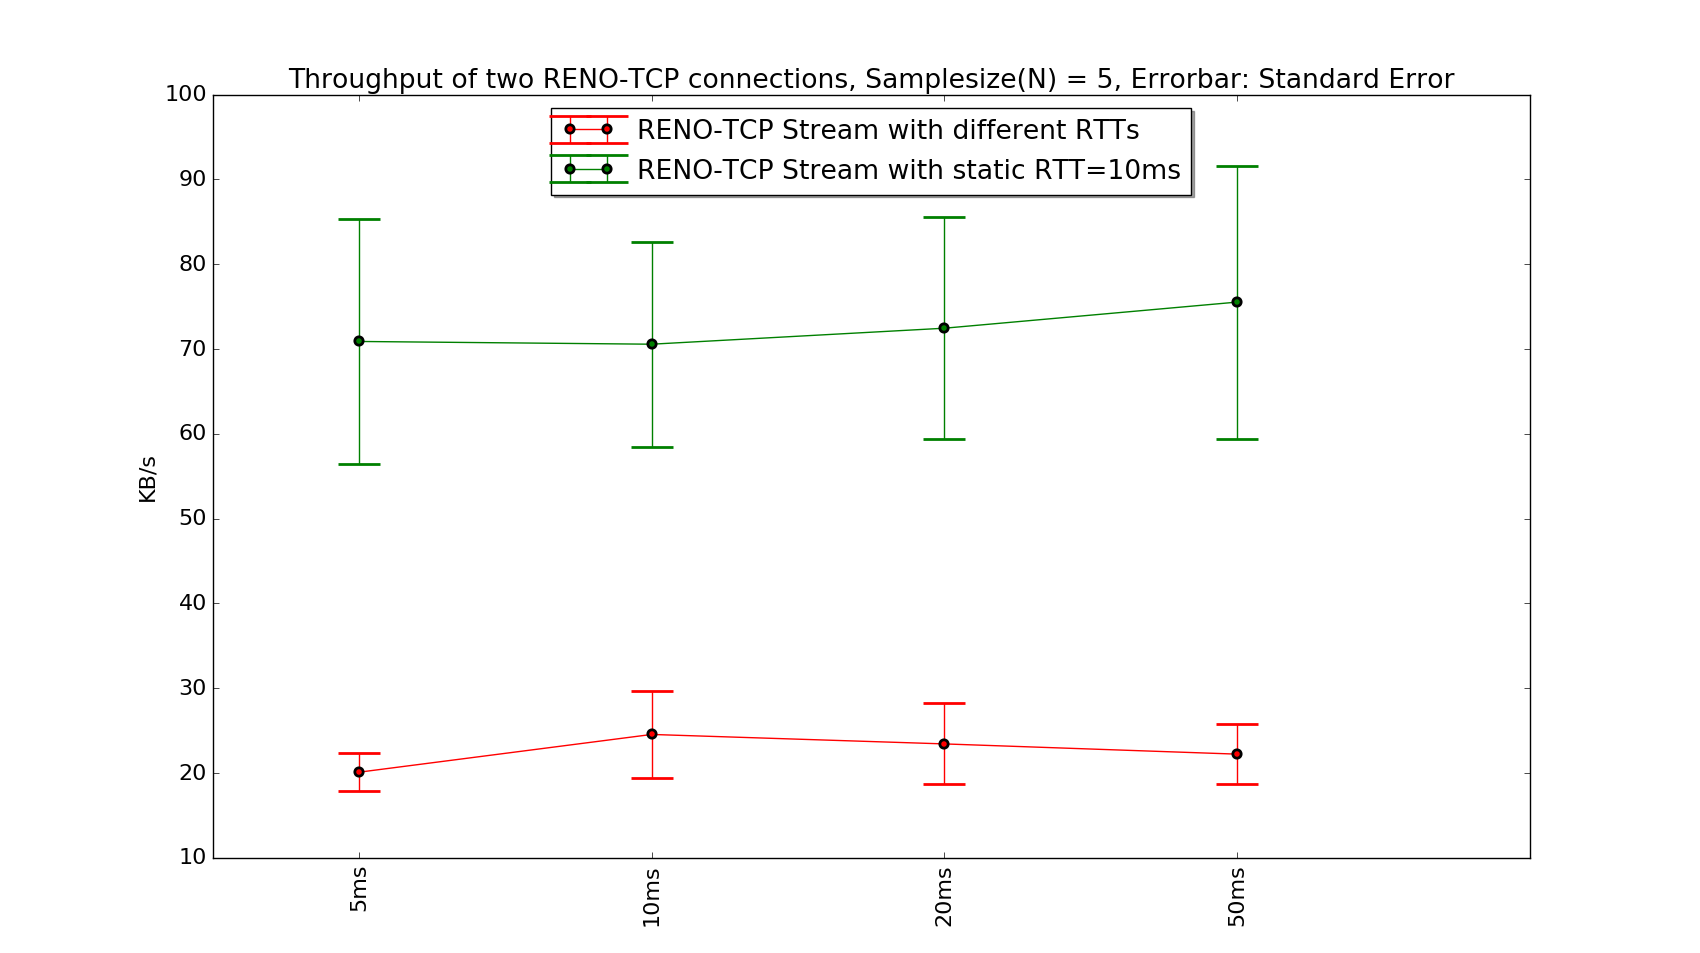
\includegraphics[width=6in]{img/reno.png}
	\caption[reno]
	{Comparision of throughput of two TCP Reno connections.}
\end{figure}

As we can see in the figure 2, the two Reno connections do not converge to a fair usage of the availabe bandwith. Instead, the TCP connection sending from node B over link $L2$ has a significantly higher throughput (around 3 times higher) compared to the TCP connection sending from node A. We would have expected, that the bandwith usage of the two TCP-NewReno connections converges to a fair usage over time. The different RTT's do not explain this strange behavior. However, we can observe that, the higher the RTT for the TCP stream sending from node A, the lower its throughput becomes and the higher the throughput of the other TCP stream becomes. This simulated behavior is predicted by our mathematical model.
\begin{table}[H]
\centering
\begin{tabular}{|l|l|l|l|}
\hline
\textbf{RTT L1} & \textbf{RTT L2} & \textbf{Corrupt Tx A} & \textbf{Corrupt Tx B} \\ \hline
5ms             & 10ms            &        16.0              &         92.4              \\ \hline
10ms            & 10ms            &         22.4              &        83.4               \\ \hline
20ms            & 10ms            &       23.6                &         68.2              \\ \hline
50ms            & 10ms            &       17.8                &         134.8              \\ \hline
\end{tabular}
\end{table}
The number of lost packages of the two TCP streams can be seen in the table above. There is no real insight to derive from the package loss here, other than it indicates that package loss is rather random and consistent. Of course the TCP flow sending from node B has roughly 3 times more package losses than the stream sending from node A, equivalent to their throughputs.

\subsubsection*{2. Case: Fairness among two Cubic-Connections}

\begin{table}[H]
\centering
\begin{tabular}{|l|l|l|l|}
\hline
\textbf{RTT L1} & \textbf{RTT L2} & \textbf{Average $Rx_A$ in KB/s} & \textbf{Average $Rx_B$ in KB/s} \\ \hline
5ms             & 10ms            &          74.08               &         72.26                \\ \hline
10ms            & 10ms            &         72.42                &           67.72              \\ \hline
20ms            & 10ms            &         69.51                &         66.37                \\ \hline
50ms            & 10ms            &          61.94               &           73.34              \\ \hline
\end{tabular}
\end{table}

We can observe in figure 3, that the two cubic connections are very efficient in sharing equal parts of bandwiths over a bottleneck link. In comparasion to the two Reno connection discussed above, the whole bandwith gets efficiently used. When we increase the RTT of one connection (The red plot in figure 3), the throughput of this connections suffers and the throughput of the competing cubic connection (the green plot in figure 3) increases. This behavior however is only starting to become visible with at a $RTT=50ms$. Additonally, we can only hypothesize that the RTT has this influence, since the differences in bandwith at $RTT=50ms$ are not significant. Furthermore, a sample size of N=5 repetitions is much too small to reliable compare two TCP streams. We should have included more simulation runs with even higher RTT's for the red connection. A good pick would have been: $latency=(5ms, 10ms, 20ms, 50ms, 100ms, 250ms, 500ms)$ to reveal bandwith patterns with rising RTT.

\begin{figure}[H]
	\centering
	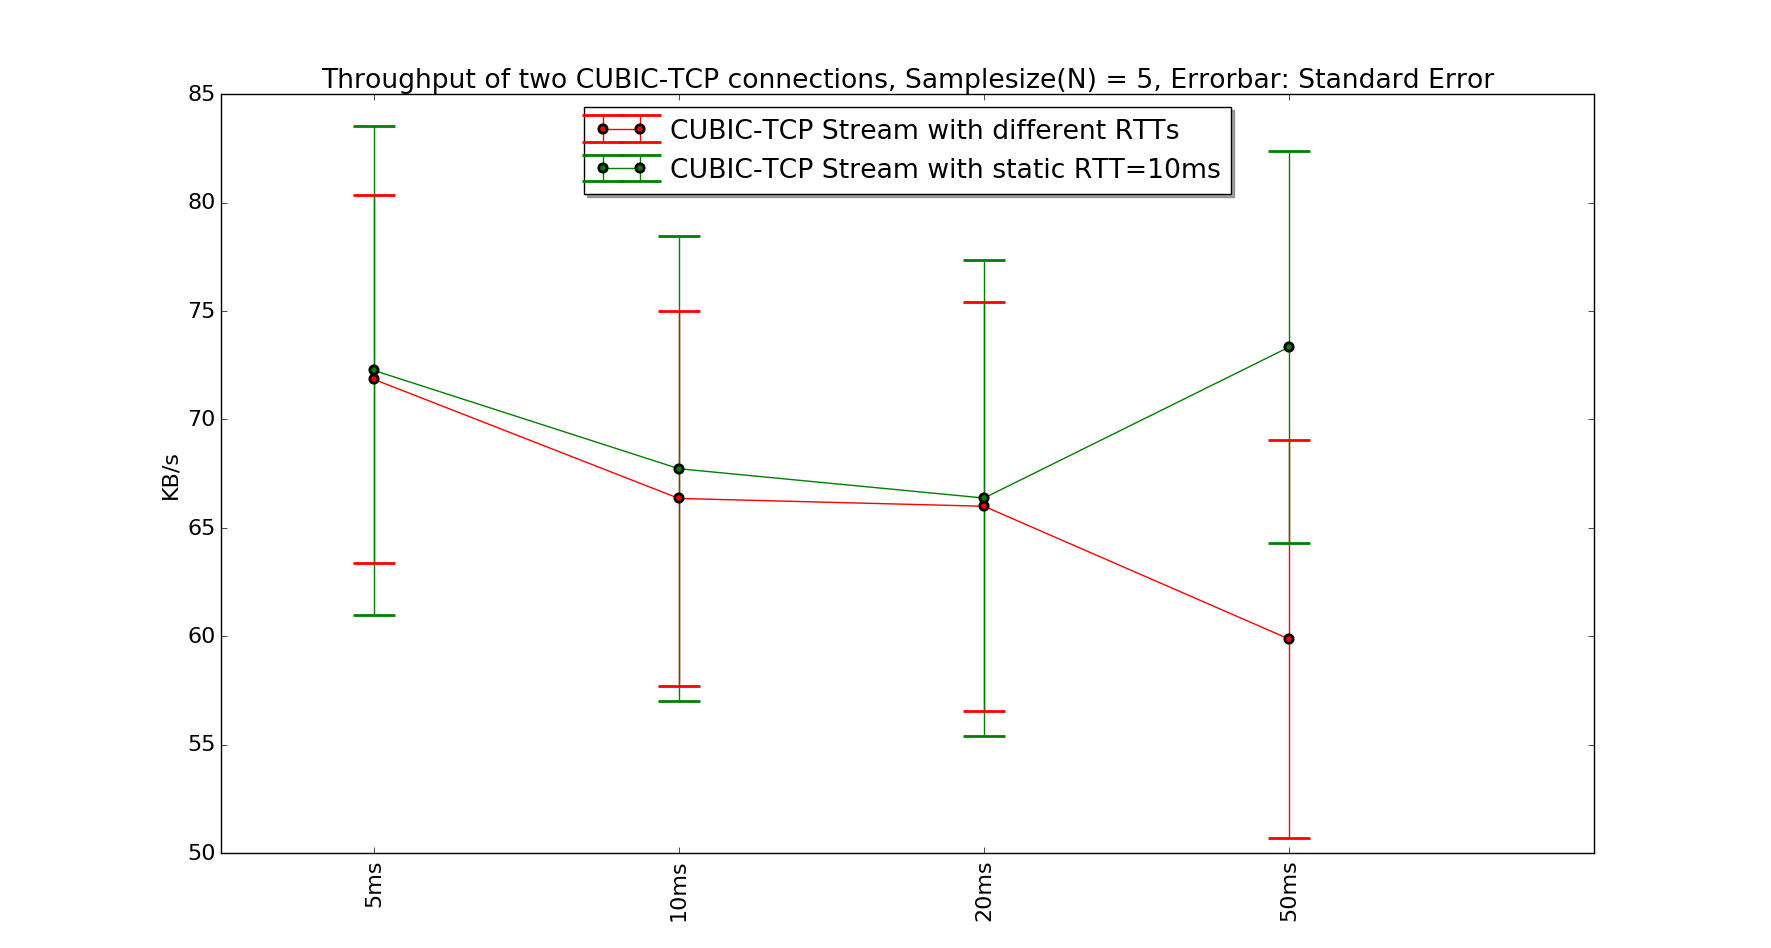
\includegraphics[width=6in]{img/cubic.png}
	\caption[reno]
	\label{fig:cubic}
	{Comparision of throughput of two Cubic connections.}
\end{figure}

The number of lost packages of the two TCP streams can be seen in the table below. As in the case with lost packages in two Reno connections, there is no additional information to be derived, other than package loss occurs on the bottleneck link.
\begin{table}[H]
\centering
\begin{tabular}{|l|l|l|l|}
\hline
\textbf{RTT L1} & \textbf{RTT L2} & \textbf{Corrupt Tx A} & \textbf{Corrupt Tx B} \\ \hline
5ms             & 10ms            &        70.0               &         112.4              \\ \hline
10ms            & 10ms            &         146.2              &        62.4               \\ \hline
20ms            & 10ms            &       85.4                &         132.8              \\ \hline
50ms            & 10ms            &       76.8                &         91.0              \\ \hline
\end{tabular}
\end{table}


\section{Conclusion} \label{conclusion}
According to the model, two competing TCP (NewReno) connections converge to a fair usage of bandwith, because if one connection currently sends more data, then this connection experiences higher losses. Additionally, because of multiplicative decrease, the faster connection loses more bandwith and converges to the same rate as the slower connection. We couldn't observe this behavior in our simulation of two NewReno connections, whereas the two cubic connections had about the same bandwith. Therefore, we are inclined to say that our simulation yielded the result, that two concurrent NewReno connections acted unfair and that cubic connections shared bandwith in a fair fashion. We assume however, that we may have introduced a non-obvious mistake in our simulation setup.\\
We expected the rate of our throughput to be  reversly proportional to their RTT: $$\frac{R_A}{R_B} = \frac{RTT_B}{RTT_A} $$ It's obvious that our data doesn't show this relationship.\\\\
Weak points of this report are the low number of sample sizes for simulation runs (N=5). Also we should have increased the RTT interval from $RTT=(5ms, 10ms, 20ms, 50ms)$ to $RTT=(5ms, 10ms, 20ms, 50ms, 100ms, 250ms, 500ms)$ to reveal underlying patters in a more significant way.


%\begin{thebibliography}{9}
%\bibitem[Doe]{doe} \emph{First and last \LaTeX{} example.},
%John Doe 50 B.C. 
%\end{thebibliography}

%%%%%%%%%%%%%%%%%%%%%%%%%%%
%         APPENDIX        % 
%%%%%%%%%%%%%%%%%%%%%%%%%%%
\let\clearpage\relax
\definecolor{listinggray}{gray}{0.9}
\definecolor{lbcolor}{rgb}{0.9,0.9,0.9}


  \lstset{
    backgroundcolor=\color{lbcolor},
    tabsize=4,
  language=C++,
  captionpos=b,
  tabsize=3,
  frame=lines,
  numbers=left,
  numberstyle=\tiny,
  numbersep=5pt,
  breaklines=true,
  showstringspaces=false,
  basicstyle=\footnotesize,
%  identifierstyle=\color{magenta},
  keywordstyle=\color[rgb]{0,0,1},
  commentstyle=\color{Darkgreen},
  stringstyle=\color{red}
  }

\newpage
\section*{Appendix} \label{appendix}

\subsection{Source Code}

The source code and simulation data for the simulation can be found in the following github repository:
\url{https://github.com/NikolaiT/PAK-Report-2}

\subsection{Applying a RateErrorModel on the bottleneck link}\label{errorModel}
\begin{lstlisting}
DoubleValue rate (err_rate);
Ptr<RateErrorModel> em1 =
  CreateObjectWithAttributes<RateErrorModel> ("RanVar",
   StringValue ("ns3::UniformRandomVariable[Min=0.0|Max=1.0]"), "ErrorRate", rate);
Ptr<RateErrorModel> em2 =
  CreateObjectWithAttributes<RateErrorModel> ("RanVar",
   StringValue ("ns3::UniformRandomVariable[Min=0.0|Max=1.0]"), "ErrorRate", rate);

thirdDevice.Get (0)->SetAttribute ("ReceiveErrorModel", PointerValue (em1));
thirdDevice.Get (1)->SetAttribute ("ReceiveErrorModel", PointerValue (em2));
\end{lstlisting}

\end{document}
